%
\documentclass[%
 reprint,
 amsmath,amssymb,
 aps,
]{revtex4-1}

\usepackage{graphicx}% Include figure files
\usepackage{dcolumn}% Align table columns on decimal point
\usepackage{bm}% bold math


\begin{document}



\title{Comparación BD NoSQL}
\author{Yaneth Virginia Aquino Huallpa}
\author{Arlyn Cotrado Coaquira}
\author{Sharon Sosa Bedoya}
\author{Marlon Villegas Arando}
\affiliation{%
 Universidad Privada de Tacna \textbackslash Facultad de Ingenieria \textbackslash Escuela Profesional de Ingenieria de Sistemas
}%


\begin{abstract}
\begin{center}
\textbf{Resumen}
\end{center}

En el presente articulo se relata la comparación hecha de bases de datos NoSQL, describiéndolas y analizando su importancia, así como las definiciones de tipos de bases de datos NoSQL, con el fin de proporcionar un punto de partida para los trabajos en esta área. Y también la creación de una base de datos, inserción y consultas de datos NoSQL mediante Docker.\\

\textbf{Palabras clave:}   NoSQL, Bases de datos, Docker.\\

\begin{center}
\textbf{Abstract}
\end{center}
In the present article the comparison made of NoSQL databases is described, describing them and analyzing their importance, as well as the definitions of NoSQL database types, in order to provide a starting point for work in this area. And also the creation of a database, insertion and queries of NoSQL data through Docker.\\
\textbf{Keywords:}  NoSQL, Databases, Docker.\\

\end{abstract}



\maketitle

%\tableofcontents

\section {Introducción}\label{sec:1}

Dia a día el manejo de la información se hace más complejo; diferentes factores hacen que las personas involucradas en el área busquen tecnologías que le ayuden con este problema. Las bases de datos relacionales son las mas comunes, pero en los últimos años ha aumentado el interés por las bases de datos NoSQL (Not only SQL), un nuevo conjunto de tecnologías que pueden contribuir al manejo de información.
\par Por lo anterior, el presente documento hace una revisión de las tecnologías NoSQL, haciendo posible hacer una comparación.\\

\par El resto de este articulo está organizado de la siguiente manera. En la Sección 2 se muestra los matriales y métodos usados para el desarrollo de este articulo. La Sección 3 se explican los resultados. Y finalmente, las conclusiones están en la Sección 4.



%-----------------------------------------------------------------
\section{Materiales y Métodos}\label{sec:2}
\subsection{Materiales}
	\begin{itemize}
		\item Virtualización activada en el BIOS
		\item Docker Desktop
		\item Windows 10 64bit: Pro, Enterprise o Education, con al menos 4GB de RAM.
	\end{itemize}
\subsection{Métodos}
	\begin{itemize}
		\item Se utilizo como material artículos y libros relacionados a la base de datos NoSQL y sus tipos, así como páginas web.
	\end{itemize}
%-----------------------------------------------------------------
\section{Marco Teórico}\label{sec:3}
\subsection{Base de datos}
	\begin{itemize}
		\item Una base de datos es una colección de datos organizados según un determinado criterio
		\item Estos datos se pueden leer, crear, actualizar y borrar
		\item También existen motores de base de datos que nos permiten hacer todas estas operaciones de forma más fácil
	\end{itemize}
\subsection{Tipos de base de datos}
	\begin{itemize}
		\item Existen distintos tipos de bases de datos que se utilizan para solucionar distintos tipos de problemas
                     \item Dentro de la gran familias de bases de datos podemos encontrar las del tipo base de datos relacionales y las no relacionales
		\item Las bases de datos relacionales se conocen generalmente como las SQL
		\item Las no relacionales se conocen como NoSQL
		\item Cada tipo de base de datos tiene beneficios y contras a la hora de almacenar, leer, actualizar o borar los datos
	\end{itemize}
\subsection{Bases de datos relacional}
	\begin{itemize}
		\item Desde su definición vemos que una base de datos puede ser relacional si cumple con algo conocido como el modelo relacional.
                     \item En la definición de modelo relacional nos podemos quedar con la idea de tablas que tienen columnas para describir los datos que están relacionados entre si.
		\item Ejemplo modelo relacional:
                     \begin{center}
		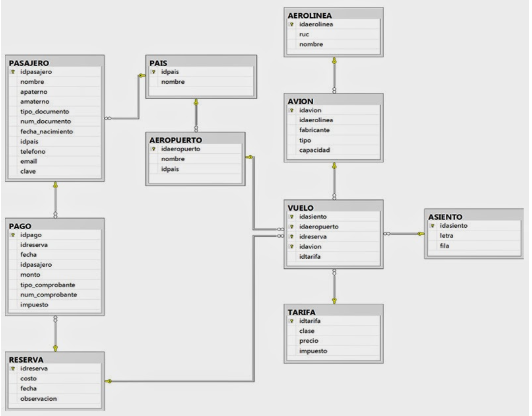
\includegraphics[width=8cm]{./Imagenes/1}
		\end{center}	
	\end{itemize}
\subsection{Modelo NoSQL}
	\begin{itemize}
		\item Se conoce como NoSQL (Not Only SQL) al grupo de bases de datos que no son relacionales
                     \item Dentro de esta clasificación se encuentran las bases de clave/valor, orientadas a documentos, grafos, de grandes columnas .
                     \begin{center}
		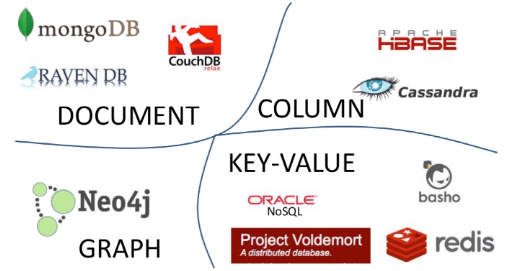
\includegraphics[width=8cm]{./Imagenes/2}
		\end{center}	
		\item Este tipo de bases de datos escala de forma horizontal
		\item Podemos utilizar muchas máquinas chiquitas para crecer y satisfacer las necesidades de los negocios actuales.
                     \begin{center}
		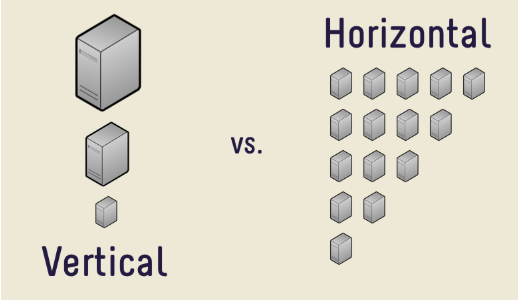
\includegraphics[width=5cm]{./Imagenes/3}
		\end{center}	
	
	\end{itemize}
%-----------------------------------------------------------------
\section {Resultados}\label{sec:4}
\subsection{Creacion de base de datos NoSQL}
\subsection{Inserción y consulta de datos}
\subsection{Comparación}
\subsection{Documental}
\subsection{Clave-Valor}
\subsection{Grafos}
\subsection{Tabular (Column-Store)}

\subsection{Comparación entre BD Documental y Clave-Valor}
		\begin{center}
		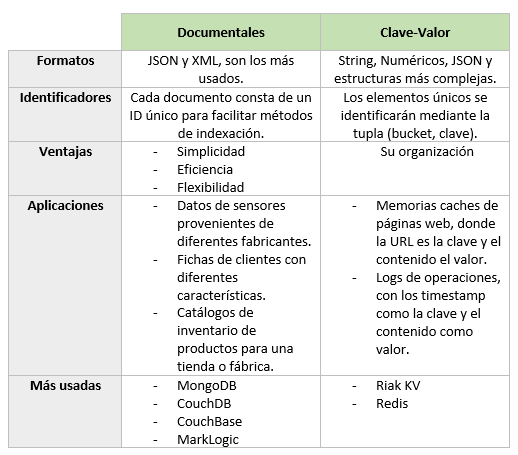
\includegraphics[width=10cm]{./Imagenes/cuadro}
		\end{center}	
%-----------------------------------------------------------------
\section{Discusión y Conclusiones}\label{sec:5}

	\begin{itemize}
		\item NoSQL permite el manejo de grandes volúmenes de datos y la posibilidad de tener un sistema distribuido.
		\item Las características de las bases de datos NoSQL responden a las necesidades actuales de las diferentes organizaciones, por lo que son una alternativa debido a su capacidad y a la velocidad.

	\end{itemize}


% Bibliografia.
%-----------------------------------------------------------------

\bibliographystyle{plain}
\bibliography{Bibliografia}

\end{document}
